% 
% Annual Cognitive Science Conference
% Sample LaTeX Paper -- Proceedings Format
% 

% Original : Ashwin Ram (ashwin@cc.gatech.edu)       04/01/1994
% Modified : Johanna Moore (jmoore@cs.pitt.edu)      03/17/1995
% Modified : David Noelle (noelle@ucsd.edu)          03/15/1996
% Modified : Pat Langley (langley@cs.stanford.edu)   01/26/1997
% Latex2e corrections by Ramin Charles Nakisa        01/28/1997 
% Modified : Tina Eliassi-Rad (eliassi@cs.wisc.edu)  01/31/1998
% Modified : Trisha Yannuzzi (trisha@ircs.upenn.edu) 12/28/1999 (in process)
% Modified : Mary Ellen Foster (M.E.Foster@ed.ac.uk) 12/11/2000
% Modified : Ken Forbus                              01/23/2004
% Modified : Eli M. Silk (esilk@pitt.edu)            05/24/2005
% Modified : Niels Taatgen (taatgen@cmu.edu)         10/24/2006
% Modified : David Noelle (dnoelle@ucmerced.edu)     11/19/2014

%% Change "letterpaper" in the following line to "a4paper" if you must.

\documentclass[10pt,letterpaper]{article}

\usepackage{cogsci}
\usepackage{pslatex}
\usepackage{apacite}
\usepackage{url}
\usepackage{graphicx}
\usepackage{caption}
\usepackage{listings}
\usepackage{color}
\usepackage{textcomp}

\graphicspath{{figures/}}


\lstset{
  language=Scheme, % Andreas Stuhlmuller. Scheme listings. https://github.com/stuhlmueller/scheme-listings.git
  columns=fixed,
  tabsize=2,
  extendedchars=true,
  breaklines=true,
  frame=single,
%  numbers=left,
  numbersep=5pt,
   basicstyle=\scriptsize\ttfamily
%  rulesepcolor=\color{solarized@base03},
%  numberstyle=\tiny\color{solarized@base01},
%  keywordstyle=\color{solarized@green},
%  stringstyle=\color{solarized@cyan}\ttfamily,
%  identifierstyle=\color{blue},
%  commentstyle=\color{solarized@base01},
%  emphstyle=\color{solarized@red}
}

\definecolor{Red}{RGB}{255,0,0}
\newcommand{\red}[1]{\textcolor{Red}{#1}}  


\title{Generic meanings are vague but rationally inferred from context}
 
 \author{{\large \bf Michael Henry Tessler, Noah D. Goodman } \\
	\{mhtessler, ngoodman\}@stanford.edu \\
  Department of Psychology, Stanford University}
 
\begin{document}

\maketitle


\begin{abstract}
Insert abstract here.

\textbf{Keywords:} 
generics; pragmatics; bayesian cognitive model; bayesian data analysis
\end{abstract}

\section{Introduction}

The meaning of generic propositions is hard to pin down. On one hand, generics would seem to suggest an almost universal quantification, as in ``Dogs bark''. Others, like ``Mosquitos carry the West Nile virus'', express a relation that applies only to a small subset of the kind. 

\citeA{Cimpian2010} (henceforth, CBG) carried out a series of studies designed to examine the truth conditions and implications of generic statements. They found evidence for the influence of context on participants' willingness to accept the relevant generics. In their paradigm, participants were given an evidence statement in terms of the percentage of a category that had a property (e.g. ``30\% of lorches have purple feathers.''). Participants were asked whether the associated generic statement (i.e. ``Lorches have purple feathers'') was true or false. The authors manipulated context by adding some additional statements about the property. In their first experiment, these extra statements either described the ``dangerousness and distinctiveness'' (e.g. ``These feathers are as sharp as needles and can easily get lodged in you, causing massive bleeding. No other animals have these kinds of feathers'') of the property or some nondangerous feature and the property's nondistinctiveness (e.g.  ``These feathers are wide and very smooth to the touch. Other animals have these kinds of feathers.''). The authors found that the dangerous and distinctive context increased the overall proportion of ``true'' responses of the generic propositions.

How are we to understand these data? One interpretation is that context changes the truth-conditions for a generic statement, but that within a context, the truth-conditions are stable. We sought out to test by doing a Bayesian data analysis of the generic truth-conditions data. 

\begin{figure}
\centering
    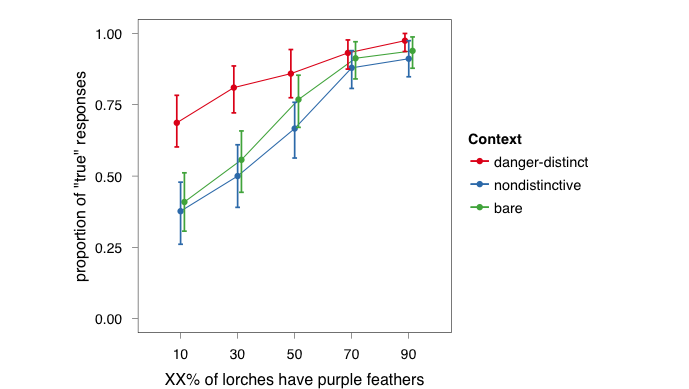
\includegraphics[width=\columnwidth]{fig1_replication}
    \caption{Replication of CBG Exp. 1, generics condition}
  \label{fig:replication}
\end{figure}

\section{Experiment 1 --- CBG (Exp. 1) replication}

Exp. 1 attempted to replicate the finding of CBG Exp. 1 that context affects the proportion of ``true'' responses to a generic statement. 

\subsection{Method}

\subsubsection{Participants}

We recruited 40 participants over Amazon's crowd-sourcing platform Mechanical Turk. 

\subsubsection{Procedure and materials}

Our procedure was identical to CBG ``truth conditions'' task, except in that our instructions were elaborated to improve interest and motivation\footnote{The experiment in full can be viewed at \url{http://stanford.edu/~mtessler/experiments/generics/cbg2010-replication/experiment/experiment-9.html}}. 

We used the same materials as CBG (available in their Appendix). The materials used were 30 novel animals (e.g. lorches, morseths, blins) each paired with a unique property. Properties were color---body-part pairs (e.g. purple feathers, orange tails). Each participant saw 10 animal-property pairs per context. Those 10 items were randomly paired with 1 of 5 ``prevalence levels'': \{10, 30, 50, 70, 90\} \%; each prevalence level appeared 2 times per context. 

Participants saw a prevalence statement and either (1) dangerous \& distinct statements, (2) control \& irrelevant statements, or (3) nothing else. Participants were asked ``Is the following sentence true or false?'', below which was presented the associated generic statement. 

\subsubsection{Results}

Our results replicated the findings of the CBG, inso far as the generic statement was endorsed more in the dangerous and distinctive context than in the other two contexts (Figure \ref{fig:replication}) \red{[insert some stats here]}. 

\section{Bayesian data analysis}

These statistics tell us that there were significantly more ``true'' responses in one context vs. another, and and that these relative proportions of ``true'' responses were most different at the lower prevalence levels. What we'd really like to know, however, is the truth-functional threshold of the generic across these three contexts. To do this, we will have to move beyond NHST to do Bayesian inference over the unknown threshold of generic. The data analysis model can be written very simply in Church.

\begin{lstlisting}
(define bayesian-data-analysis 
	(query
	
		(define generic-threshold 
			(lambda (context) (uniform 0 1)))
	
		(define generic 
			(lambda (prevalence context) 
				(> prevalence (generic-threshold context))))
				
		generic-threshold
		
		(= experiment1-data 
			(map generic all-prevalences all-contexts)))
\end{lstlisting}

Here, we say that we, as scientists, have perfect uncertainty about what the generic might mean a priori. Thus, the generic-threshold follows a uniform prior distribution between 0 and 1\footnote{If the true threshold turns out to be 0, the generic ``Lorches have purple feathers'' would mean essentially, ``Some lorches have purple feathers''. If the threshold turned out to be very close to 1, the generic would mean essentially: ``All lorches have purple feathers''.}. The generic, here, has a truth-functional meaning such that it is \lstinline{true} when the prevalence is over \lstinline{generic-threshold}, and false when it is not. The \lstinline{query} function is written to return \lstinline{generic-threshold}, which is the parameter we are interested in inferring. Finally, the last line is our condition statement: we condition on the data we collected in Experiment 1, \lstinline{map}ping appropriately over the various contexts and prevalence levels given to the participants\footnote{Technically, we must also include a guessing parameter, to account for instances when a participant responds in a contradictory manner to what the inferred threshold would imply}. 

\subsection{Results}

The results can be seen if Figure \ref{fig:bda1a}. In the ``bare'' condition, the analysis says the threshold is between 0 and 30, but is uncertain where exactly in that range the threshold would be. Critically, in the ``dangerous and distinctive'' context, the analysis infers a lower threshold, less than 10. This matches with the intuition, and the empirical results, that a dangerous and distinctive context allows for the generic to be more permissive (e.g. ``Mosquitos carry West Nile Virus'' is true, even though very few mosquitoes actually do). Finally, and most intriguingly, the analysis infers a 3rd distinct threshold profile for the nondistinctive context.  For this, it says that threshold is greater than 10, but could be as high as 50. This is an overall higher inferred threshold for the nondistinctive category, and an aspect totally missed by standard NHST. 

\begin{figure}
\centering
    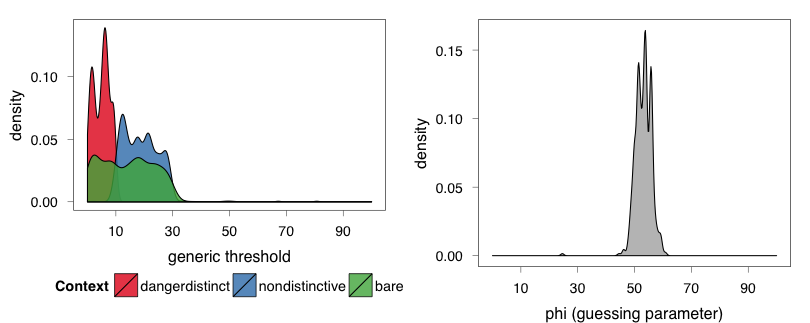
\includegraphics[width=\columnwidth]{fig2_bda1_combined}
    \caption{Inferred threshold for the generic across contexts}
  \label{fig:bda1a}
\end{figure}

There is something fundamentally wrong about this analysis, however. Specifically, there is a problem with the cognitive model. The model is a simple model of truth-functional semantics, stating that any situation with a prevalence greater than the threshold will return True, and anything less, will return False. We see the consequences of these assumptions in the data analysis parameter $\phi$. $\phi$ represents the percentage of responses that the data analysis model wants to attribute to guessing. This proportion is somewhere between 40 and 50\%. The amount of guessing is so high because our computational model is inflexible.




This can also be seen in the posterior predictive distribution of responses. The model matches the trajectory of the dangerous \& distinct context reasonably well, but is too dichotomous in the other contexts. The correlation between the posterior predictive and the data is $r = 0.86$. 

\begin{figure}
\centering
    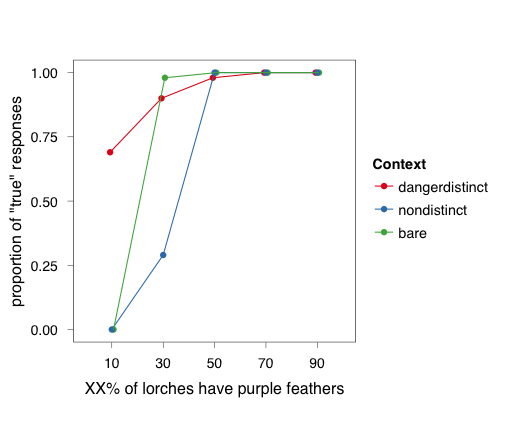
\includegraphics[width=\columnwidth]{fig3_bda1_postpred}
    \caption{Posterior predictive using fixed-threshold semantics}
  \label{fig:bda1posteriorpred}
\end{figure}





%\begin{itemize}
%\item Inferred value of theta across contexts. 
%\item $\phi$ parameter. 
%\item Posterior predictive of fixed threshold model?

Rather than just say context gives rise to different thresholds, we should instead consider that the threshold is \emph{actively inferred}, by the subject, from context. This gives rise to a slightly different type of model... a cognitive, language-understanding model.

%\end{itemize}

\section{Lifted-variable RSA}

The bayesian data analysis above provides evidence that context influences the truth-conditions of a generic statement. The poor qualitative fit as well as the inferred value of the guessing parameter $\phi$ suggest, however, that our model of cognition is incomplete. Rather than propose that the meaning of a generic is simply a one-to-one mapping between context and threshold, we propose people have uncertainty about the true threshold and actively reason about this meaning from context. 

To formalize this, we draw on work from the Rational Speech-Act (RSA) theory of communication \cite{Frank2012}. In this framework, a listener infers the meaning of an utterance by a recursive reasoning process, wherein she considers the thought-processes of a speaker whose goal is to be informative. This theory has had tremendous support for providing quantitative predictions of a number of linguistic phenomena including scalar implicature, hyperbole, and multiple classes of reasoning paradigms \cite{Goodman2013, Kao2014, Tessler2014, Lassiter2014}. 

\citeA{Lassiter2015} proposed an elaboration of the theory to account for interpreting vague, gradable adjectives like \emph{tall}. They propose the meaning of an adjective like \emph{tall} is a standard truth-functional meaning such that the adjective is true if the object in question has a height greater than the threshold $\theta_{tall}$. The suggestion, though, is that the listener has uncertainty about what $\theta_{tall}$ actually is, and infers that value of $\theta_{tall}$ via the same recursive reasoning process. Here, we borrow the same formalism to try account for the uncertainty in generic meaning.

In Church, the model looks like

\begin{lstlisting}
(define rational-speech-act


	(define pragmatic-listener
		(lambda (utterance)
			(define state (state-prior))
			(define generic-theta (theta-prior))
			
			generic-theta
			
			(equal? utterance (speaker state generic-theta))))
			
	(define speaker 
		(lambda (state generic-theta)
			(define utterance (utterance-prior))
			
			utterance
			
			(equal? state (literal-listener utterance generic-theta))))
			
	(define literal-listener
		(lambda (utterance generic-theta)
			(define state (state-prior))
			
			state
			
			(utterance state generic-theta))))
\end{lstlisting}

We propose that the subject in this task is actively reasoning about the threshold, i.e. the truth-conditions of the generic. Note how this is different from the previous model, wherein the subject is presumed to already know the threshold, and that she just has to look it up what it is in the context--to--threshold mapping. 

Now, how is the subject supposed to reason about the threshold? We propose that the subject reasons about the threshold via the contextual information given to her. In CBG, this contextual information are the 3 conditions: \emph{dangerous and distinct}, \emph{nondistinct}, and \emph{bare}. In this simple model, the contextual information could provide different \lstinline{state-prior} distributions. \lstinline{state-prior} represents the percentage of the kind that has the property. Naively, this would be \lstinline{(uniform 0 1)}, or equivalently \lstinline{(beta 1 1)}. However, we propose that the subject doesn't know exactly what this prior distribution over states looks like. We put uncertainty over the parameters of this beta distribution, \lstinline{(beta gamma delta)}\footnote{For ease of interpretation, we are parametrizing the \lstinline{beta} distribution by its mean and some measure of its variability ... \lstinline{(beta (* gamma delta) (* (- 1 gamma) delta))}} 

Thus, we put a bayesian data analysis model over our Rational Speech-Act model of language understanding, to see how context might influence the prior distribution. In Church, this looks like

\begin{lstlisting}
(define the-full-bayesian-thing
	(query
	
		(define gamma
			(lambda (context) (uniform 0 1)))
			
		(define delta
			(lambda (context) (uniform 0 5)))
	
		(define rational-speech-act
			(lambda ( (gamma context) (delta context) ) 
				...))
				
		'((map gamma all-contexts) (map delta all-contexts))
		
		(= experiment1-data 
			(map rational-speech-act all-prevalences all-contexts))))
\end{lstlisting}

\begin{figure}
\centering
    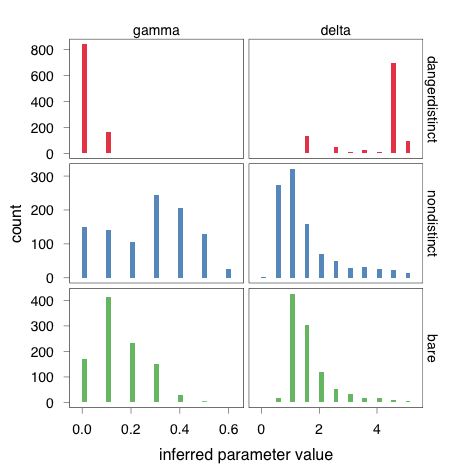
\includegraphics[width=\columnwidth]{fig4_bda2_hyper}
    \caption{Hyperprior parameters for lifted-variable RSA model}
  \label{fig:bda2hyperparams}
\end{figure}

We can examine the inferred hyperprior parameter values for the Lifted-variable RSA model. $\gamma$ is a measure of central tendency, and of primary concern for this analysis. We can see that if this were the correct model of human cognition, the prior probability of the \emph{dangerous \& distinctive} condition would be heavily skewed towards lower prevalence levels. This makes sense insofar as a distinctive feature is one that is relatively rare. Our intuitions are again confirmed in the inferred distribution of the \emph{nondistinctive} context. A nondistinctive feature is one that is very common. The prior distribution of the \emph{bare} context lies somewhere in between these two extremes: neither distinctive nor nondistinctive.




The posterior predictive distributions marginalizes over the hyperprior parameters. The predictions for the lifted variable RSA model are in Figure \ref{fig:postpred2}. We can see here that model has some persistent uncertain about what the true threshold is and this is manifested in its intermediate endorsement rates for the generic at lower prevalence levels. We reconstruct the curves of Figure \ref{fig:replication} well; the model--data correlation is $r = 0.97$. 

\begin{figure}
\centering
    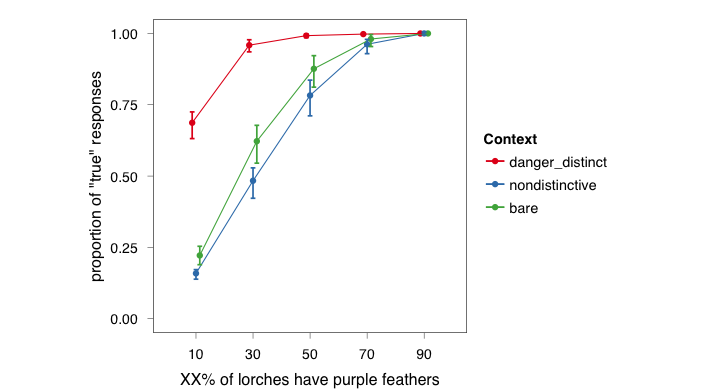
\includegraphics[width=\columnwidth]{fig5_bda2_postpred}
    \caption{Posterior predictive using lifted-variable RSA}
  \label{fig:postpred2}
\end{figure}

In addition to making predictions about the proportion of ``true'' responses to generic statement under different prevalence levels, the combination of the bayesian model of language understanding and the bayesian data analysis model gives rise to predictions about the shape of the prior distribution of prevalence levels under different contexts. We take these predictions seriously, and test these in a second experiment. 

\section{Experiment 2}

Exp. 2 sought to test the prediction that the prior distribution of prevalence levels would vary by context, as predicted by the $\gamma$ and $\delta$ data analysis parameters from the previous section.

\subsection{Method}

\subsubsection{Participants}

We recruited 30 participants over Amazon's crowd-sourcing platform Mechanical Turk. 

\subsubsection{Procedure and materials}

Our procedure was identical to Experiment 1 in all aspects except the question that was asked of the participant\footnote{The experiment in full can be viewed at \url{http://stanford.edu/~mtessler/experiments/generics/cbg2010-replication/experiment/experiment-8.html}}. 

Participants were presented with the following piece of information ``The island has 100,000 other animals on it.'' and asked the following question: ``How many other animals do you think have purple feathers?''

\subsubsection{Results}



\begin{itemize}

\item Replace figure 4 (hyperprior parameters) with mean distribution?

\item Collapse Figure 3 \& 5 (posterior predictive) into one

\item Exp 2 to confirm $\gamma$ and $\delta$. 

\item Some linking function to condition on Exp 1 \& 2 simultaneously,  to perhaps, infer rationality parameter and get some posterior predictives.

\end{itemize}
%They also performed analyses testing the relation between two dependent measures for understanding generics. In this latter analysis, they found that the quantifier ``most'' expressed a symmetry between these two dependent measures, while the generic had an asymmetry \footnote{This asymmetry has also been replicated in adults and observed in children \cite{Brandone2014}}.

%The data analysis involved comparing the mean of the prevalence ratings associated with \emph{True} endorsements of the generic with the mean prevalence ratings elicited by the generic in a separate task. In the experimental pragmatics literature, the dependent measure involved in the ``truth conditions'' task is called \emph{sentence verification}; in the ``implied prevalence'' task, it is a \emph{sentence interpretation}. 
%
%These different dependent measures, we argue, imply different Questions Under Discussion (QUD, \cite{Roberts2004}). 



%	\section{Sentence verification is a speaker task}
%	
%	DegenGoodman2014.  Truth conditions task --> QUD = ``generic true?'' Model.
%	
%	But what is the semantics of the generic? \citeA{Cimpian2010}, experiments 1, 3, and 4 found that the truth conditions of the generic are sensitive to the context.  Our goal is to replicate this finding, and use Bayesian data analysis to infer the threshold of the speaker model. This bears some similarity to Michael Franke's approach for cogsci from last year.
%	
%	
%	
%	
%	\section{The full bayesian thing}
%	
%	Computational models of cognition typically have parameters. Many of these parameters are of theoretically interest, because they are posited to reside within the head of the subject.
%	
%	\subsection{Inferring quantifier threshold by context}
%	
%	Here we'll find that the generic threshold changes by context. We might also want to show that ``most'' and ``some'' do not change by context.
%	
%	\subsection{Are generics like adjectives?}
%	
%	To determine if a generic is true or false, we must refer to context. The threshold in the threshold-semantic view of the statement varies by context. This property has been shown to be an important feature in the semantics of gradable adjectives (e.g. \emph{tall}) \cite{Lassiter2014}.  
%	
%	\section{Lifted-variable speech act model}
%	
%	We can start in a single context, with a uniform prior over states. We can look at the posterior over states, for listener1. As well, we can look at the posterior over thetas. This depends of course on the alternatives, for which we may want to consider only the experimental alternatives \emph{some, most, generic} or for which we may want to include \emph{all}.  Either way, here we'll recreate the asymmetry between listener and speaker --- between implied prevalence and truth conditions. 
%	
%	\citeA{Cimpian2010} report a ``paradoxical asymmetry at the core of generic meaning'' which manifests as the generic having ``extremely strong implications but requiring little evidence to be judged true''. Here, we explain this ``paradox'' by the different Questions Under Discussions in the tasks used and by the different roles intrinsic to speech-acts: the role of the speaker and the role of the listener. 
%	
%	\subsection{Questions Under Discussion in two tasks}
%	
%	\citeA{Cimpian2010} used two tasks (with different dependent measures) to get at the comparison between ``acceptance'' and ``implications''. These two tasks --- called ``truth conditions'' and ``implied prevalence'' -- used different questions and different dependent measures to get at the meaning of generics. In the ``truth conditions'' task, subjects are given evidence about the prevalence of a property (e.g. ``50\% of morseths have silver fur'') and are asked to judge the corresponding generic (i.e. ``Morseths have silver fur'') to be either true or false. In the ``implied prevalence'' task, subjects are given a generic statement and asked ``What percentage of morseths do you think have silver fur?''
%	
%	\citeA{Degen2014} argue that the \emph{sentence verification} (``truth conditions'') task should be modeled as a speaker task, and that the \emph{sentence interpretation} (``implied prevalence'') task should be modeled as a listener task. In addition to different communicative roles, there are also different implicit Questions Under Discusision. In the ``truth conditions'' task, the QUD seems to be ``is the generic true or false?'', whereas in the ``implied prevalence'' task, the QUD seems to be ``what percentage of category X have property Y?''.







%
%\section{General Formatting Instructions}
%
%The entire contribution of a proceedings paper (including figures,
%references, and anything else) can be no longer than six pages.
%
%The text of the paper should be formatted in two columns with an
%overall width of 7 inches (17.8 cm) and length of 9.25 inches (23.5
%cm), with 0.25 inches between the columns. Leave two line spaces
%between the last author listed and the text of the paper. The left
%margin should be 0.75 inches and the top margin should be 1 inch.
%\textbf{The right and bottom margins will depend on whether you use
%  U.S. letter or A4 paper, so you must be sure to measure the width of
%  the printed text.} Use 10~point Times Roman with 12~point vertical
%spacing, unless otherwise specified.
%
%The title should be in 14~point, bold, and centered. The title should
%be formatted with initial caps (the first letter of content words
%capitalized and the rest lower case). Each author's name should appear
%on a separate line, 11~point bold, and centered, with the author's
%email address in parentheses. Under each author's name list the
%author's affiliation and postal address in ordinary 10~point type.
%
%Indent the first line of each paragraph by 1/8~inch (except for the
%first paragraph of a new section). Do not add extra vertical space
%between paragraphs.
%
%
%\section{First Level Headings}
%
%First level headings should be in 12~point, initial caps, bold and
%centered. Leave one line space above the heading and 1/4~line space
%below the heading.
%
%
%\subsection{Second Level Headings}
%
%Second level headings should be 11~point, initial caps, bold, and
%flush left. Leave one line space above the heading and 1/4~line
%space below the heading.
%
%
%\subsubsection{Third Level Headings}
%
%Third level headings should be 10~point, initial caps, bold, and flush
%left. Leave one line space above the heading, but no space after the
%heading.
%
%
%\section{Formalities, Footnotes, and Floats}
%
%Use standard APA citation format. Citations within the text should
%include the author's last name and year. If the authors' names are
%included in the sentence, place only the year in parentheses, as in
%\citeA{NewellSimon1972a}, but otherwise place the entire reference in
%parentheses with the authors and year separated by a comma
%\cite{NewellSimon1972a}. List multiple references alphabetically and
%separate them by semicolons
%\cite{ChalnickBillman1988a,NewellSimon1972a}. Use the
%``et~al.'' construction only after listing all the authors to a
%publication in an earlier reference and for citations with four or
%more authors.
%
%
%\subsection{Footnotes}
%
%Indicate footnotes with a number\footnote{Sample of the first
%footnote.} in the text. Place the footnotes in 9~point type at the
%bottom of the column on which they appear. Precede the footnote block
%with a horizontal rule.\footnote{Sample of the second footnote.}
%
%
%\subsection{Tables}
%
%Number tables consecutively. Place the table number and title (in
%10~point) above the table with one line space above the caption and
%one line space below it, as in Table~\ref{sample-table}. You may float
%tables to the top or bottom of a column, or set wide tables across
%both columns.
%
%\begin{table}[!ht]
%\begin{center} 
%\caption{Sample table title.} 
%\label{sample-table} 
%\vskip 0.12in
%\begin{tabular}{ll} 
%\hline
%Error type    &  Example \\
%\hline
%Take smaller        &   63 - 44 = 21 \\
%Always borrow~~~~   &   96 - 42 = 34 \\
%0 - N = N           &   70 - 47 = 37 \\
%0 - N = 0           &   70 - 47 = 30 \\
%\hline
%\end{tabular} 
%\end{center} 
%\end{table}
%
%
%\subsection{Figures}
%
%All artwork must be very dark for purposes of reproduction and should
%not be hand drawn. Number figures sequentially, placing the figure
%number and caption, in 10~point, after the figure with one line space
%above the caption and one line space below it, as in
%Figure~\ref{sample-figure}. If necessary, leave extra white space at
%the bottom of the page to avoid splitting the figure and figure
%caption. You may float figures to the top or bottom of a column, or
%set wide figures across both columns.
%
%\begin{figure}[ht]
%\begin{center}
%\fbox{CoGNiTiVe ScIeNcE}
%\end{center}
%\caption{This is a figure.} 
%\label{sample-figure}
%\end{figure}
%
%
%\section{Acknowledgments}
%
%Place acknowledgments (including funding information) in a section at
%the end of the paper.
%
%
%\section{References Instructions}
%
%Follow the APA Publication Manual for citation format, both within the
%text and in the reference list, with the following exceptions: (a) do
%not cite the page numbers of any book, including chapters in edited
%volumes; (b) use the same format for unpublished references as for
%published ones. Alphabetize references by the surnames of the authors,
%with single author entries preceding multiple author entries. Order
%references by the same authors by the year of publication, with the
%earliest first.
%
%Use a first level section heading, ``{\bf References}'', as shown
%below. Use a hanging indent style, with the first line of the
%reference flush against the left margin and subsequent lines indented
%by 1/8~inch. Below are example references for a conference paper, book
%chapter, journal article, dissertation, book, technical report, and
%edited volume, respectively.
%
%\nocite{ChalnickBillman1988a}
%\nocite{Feigenbaum1963a}
%\nocite{Hill1983a}
%\nocite{OhlssonLangley1985a}
%% \nocite{Lewis1978a}
%\nocite{Matlock2001}
%\nocite{NewellSimon1972a}
%\nocite{ShragerLangley1990a}
%

\bibliographystyle{apacite}

\setlength{\bibleftmargin}{.125in}
\setlength{\bibindent}{-\bibleftmargin}

\bibliography{generics}


\end{document}
